\documentclass{math}

\usepackage{tikz}

\title{University Physics 2}
\author{Alvin Lin}
\date{January 2018 - May 2018}

\begin{document}

\maketitle

\section*{Electric Flux}
Light, magnetism, heat, and water can all have flux. Flux is defined as the flow
of some field through a surface.
\[ \Phi_{E} = \vec{E}\cdot\vec{A} \]
\[ \vec{A} = A\vec{n} \]
\( \vec{A} \) is an area centered on the surface, with the magnitude equal to
the area and the direction pointing normal to the surface. For a figure with
multiple surfaces:
\[ \Phi_E = \sum\vec{E}\cdot\Delta\vec{A} \]
Gauss's Law states that the electric flux through a closed surface is
proportional to the charge inside the surface (denoted \( Q_{enc} \)).
\[ \Phi_E = \frac{Q_{enc}}{\epsilon_{\circ}} \quad
  K = \frac{1}{4\pi\epsilon_{\circ}} \]
\[ \Phi_E = \oint\vec{E}\cdot\diff{\vec{A}} =
  \frac{Q_{enc}}{\epsilon_{\circ}} \]

\subsection*{Gauss's Law for a Point Charge}
\begin{center}
  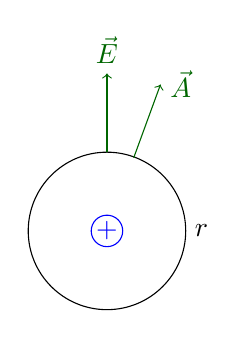
\begin{tikzpicture}
    \draw[blue] (0,0) circle (0.2cm) node {+};
    \draw (0,0) circle (1cm) node[xshift=1.2cm] {\( r \)};
    \draw[->,black!60!green] (0,1) -- (0,2) node[above] {\( \vec{E} \)};
    \draw[->,black!60!green] (0.34,0.93) -- (0.68,1.86)
      node[right] {\( \diff{\vec{A}} \)};
  \end{tikzpicture}
\end{center}
Use Gauss's Law to find \( \vec{E} \) at \( r \) given a point charge surrounded
by a spherical shell of radius \( r \):
\begin{align*}
  \oint\vec{E}\cdot\diff{\vec{A}} &= \frac{Q_{enc}}{\epsilon_{\circ}} \\
  &= \oint|E||\diff{\vec{A}}|\cos\theta \\
  \theta &= 0 \text{ via spherical symmetry} \\
  &= \oint|E||\diff{\vec{A}}| \\
  &= |E|\oint|\diff{\vec{A}}| \text{ since } E \text{ is constant over } r \\
  &= |E|4\pi r^2 \\
  |E|4\pi r^2 &= \frac{Q}{\epsilon_{\circ}} \\
  |E| &= \frac{1}{4\pi r^2}\frac{Q}{\epsilon_{\circ}} \text{ (Coulomb's Law)}
\end{align*}

\subsection*{Solving Gauss's Law}
\begin{enumerate}
  \item Draw a picture with axes, distances, coordinates, \( \diff{q} \),
  \( \vec{E} \) fields, \( \diff{\vec{A}} \).
  \item Decide how to solve the problem. For 3D symmetric charge distribution,
  use Gauss's Law. For 2D rings or lines, use the integral form of Coulomb's
  Law.
  \item Pick a Gaussian surface. For objects with spherical symmetry, use a
  shell. For objects with cylindrical symmetry, use a hollow cylinder. For
  objects with planar symmetry, use a box or cylinder.
  \item Write Gauss's Law:
  \[ \oint\vec{E}\cdot\diff{\vec{A}} = \frac{Q_{enc}}{\epsilon_{\circ}} \]
  \item Use symmetry to solve the left hand side. Always pick a Gaussian surface
  so that \( \vec{E} \) is parallel to \( \diff{\vec{A}} \) so that
  \( \vec{E}\cdot\diff{\vec{A}} = |\vec{E}||\diff{\vec{A}}| \).
  \item Also argue via symmetry that \( |\vec{E}| \) is independent of
  integrating variables so that \( \int|\vec{E}||\diff{\vec{A}}| =
  |\vec{E}|\oint\diff{\vec{A}} \).
  \item Solve the integral for the area. \( |\vec{E}|\oint\diff{\vec{A}} =
  |\vec{E}|A \). For a shell, \( A = 4\pi r^2 \). For the side of a cylindrical
  surface, \( A = 2\pi rh \). For the top and bottom of a cylindrical surface,
  \( A = \pi r^2 \).
  \item Calculate \( Q_{enc} \), this can be easy or hard depending on the
  problem. Remember that \( Q = \rho V \).
  \item Solve for \( |\vec{E}| \).
\end{enumerate}

\begin{center}
  You can find all my notes at \url{http://omgimanerd.tech/notes}. If you have
  any questions, comments, or concerns, please contact me at
  alvin@omgimanerd.tech
\end{center}

\end{document}
